\documentclass[tikz,border=6pt]{standalone}
\usepackage[utf8]{inputenc}
\usepackage{xcolor}
\usepackage{amsmath}
\usetikzlibrary{arrows.meta,calc,positioning,fit}
\renewcommand{\familydefault}{\sfdefault}

\definecolor{medBlue}    {HTML}{4A86B8}
\definecolor{resnetGreen}{HTML}{6FA888}
\definecolor{loss1}      {HTML}{F1D897}
\definecolor{panelGray}  {HTML}{CFCFCF}

\tikzset{
  font=\sffamily\footnotesize,
  arrow/.style={-{Latex[length=2.2mm,width=1.7mm]},draw=black,line width=1.0pt},
  panel/.style={rounded corners=8pt,draw=panelGray,dashed,line width=1.2pt,fill=white},
  model/.style={rectangle,rounded corners=3pt,draw=none,fill=medBlue,text=white,
    minimum width=4.0cm,minimum height=1.5cm,align=center,inner xsep=6pt,font=\bfseries\footnotesize},
  resnet/.style={rectangle,rounded corners=3pt,draw=none,fill=resnetGreen,text=white,
    minimum width=4.0cm,minimum height=1.5cm,align=center,inner xsep=6pt,font=\bfseries\footnotesize},
  data/.style={rectangle,rounded corners=3pt,draw=black!50,line width=0.9pt,fill=black!6,
    minimum width=4.0cm,minimum height=1.4cm,align=center,inner xsep=6pt,font=\scriptsize\itshape},
  outbox/.style={rectangle,draw=none,minimum width=4.0cm,minimum height=1.3cm,
    align=center,inner xsep=6pt,font=\bfseries\scriptsize},
  title/.style={font=\sffamily\bfseries\large,align=center},
}

\begin{document}
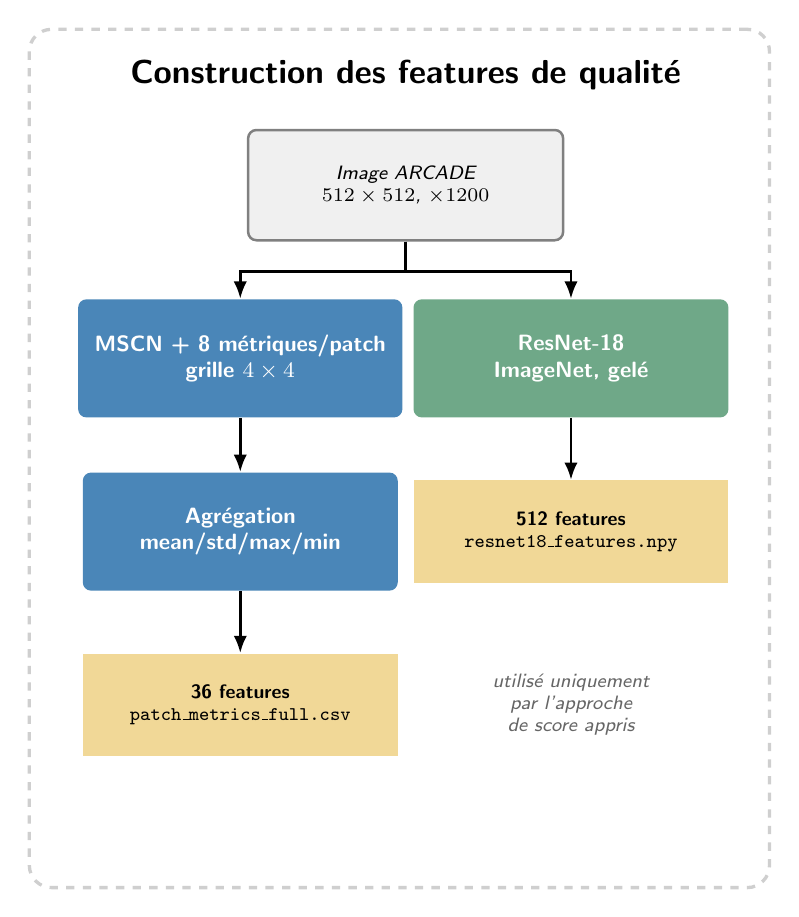
\begin{tikzpicture}[x=1cm,y=1cm]

\node[panel,minimum width=9.4cm,minimum height=10.9cm,anchor=north west] at (-.3,14.8){};

\node[title] at (4.5,14.2) {Construction des features de qualit\'e};

\node[data] (img) at (4.5,12.8) {Image ARCADE\\$512\times512$, $\times1200$};

\node[model]  (mscn)   at (2.4,10.6) {MSCN + 8 m\'etriques/patch\\grille $4\times4$};
\node[resnet] (resnet) at (6.6,10.6) {ResNet-18\\ImageNet, gel\'e};

\draw[arrow] (img.south) -- (4.5,11.7) -- (2.4,11.7) -- (mscn.north);
\draw[arrow] (img.south) -- (4.5,11.7) -- (6.6,11.7) -- (resnet.north);

\node[model]  (agg)      at (2.4,8.4) {Agr\'egation\\mean/std/max/min};
\node[outbox,fill=loss1] (feat512) at (6.6,8.4) {512 features\\\texttt{resnet18\_features.npy}};

\draw[arrow] (mscn.south)   -- (agg.north);
\draw[arrow] (resnet.south) -- (feat512.north);

\node[outbox,fill=loss1] (feat36) at (2.4,6.2) {36 features\\\texttt{patch\_metrics\_full.csv}};

\draw[arrow] (agg.south) -- (feat36.north);

\node[font=\sffamily\scriptsize\itshape,text=black!60,align=center] at (6.6,6.2)
  {utilis\'e uniquement\\par l'approche\\de score appris};

\end{tikzpicture}
\end{document}
